\documentclass{beamer}
\usepackage[utf8]{inputenc}
\usepackage[T1]{fontenc}
\usepackage{textpos}

\title{AMIDST \\ \Large \textcolor{orange!60}{Analysis} 
				   \textcolor{blue!50!cyan!80}{of MassIve} 
				   \textcolor{olive!5!green!90}{Data STreams}}
\subtitle{Requirement Engineering for a Small Project with Pre-Specified Scope} 
\author{{\scriptsize Thomas D.\ Nielsen$^{1}$, Sigve Hovda$^{2}$, Antonio Fern\'andez$^{3}$, \\ Helge Langseth$^{2}$, 
Anders L.\ Madsen$^{4}$, \\Andr\'es Masegosa$^{2}$ and  Antonio Salmer\'on$^{3}$ \\
 $^{1}$Univeristy of Aalborg, $^{2}$Norwegian University of Science and Technology, 
\\
 $^{3}$Universidad de Almeria, $^{4}$Hugin Expert}}


%
%\author{Sigve Hovda}
%\institute{Postdoctoral Fellow, Norwegian University of Science and Technology \\
%Principal Research Engineer, Verdande Technology}
\date{Fredrikstad, November 18, 2014}

\usetheme{amidst}


\AtBeginSection[]
{
   \begin{frame}
       \frametitle{Outline}
       \vspace{-1cm}
       \tableofcontents[currentsection]
   \end{frame}
}


\begin{document}

%---------------------------------------------------------------------------------------------
\begin{frame}\frametitle{}
\titlepage
\end{frame}

%---------------------------------------------------------------------------------------------
\begin{frame}\frametitle{Outline}
\vspace{-1cm}
\tableofcontents
\end{frame}
%---------------------------------------------------------------------------------------------

%%%%%%%%%%%%%%%%%%%%%%%%%%%%%%%%%%%%
\section{Introduction of the AMIDST Project}
%%%%%%%%%%%%%%%%%%%%%%%%%%%%%%%%%%%%

%---------------------------------------------------------------------------------------------

\begin{frame} \frametitle{The AMIDST Project} 
\vspace{-1cm}

\begin{itemize}
\item<1-> Research project:
\begin{itemize}
\item<1-> Funded by the EU seventh programme
\end{itemize}
\item<2-> Objective: 
\begin{itemize}
\item<2-> Toolbox that facilitates efficient prediction and data analysis in streaming data
\end{itemize}
\item<3-> Consortium:
\begin{itemize}
\item<3-> Three academic partners
\begin{itemize}
\item<3-> Univeristy of Aalborg
\item<3-> Norwegian University of Science and Technology
\item<3-> Universidad de Almeria
\end{itemize}
\item<4-> Four industrial partners
\begin{itemize}
\item<4-> Verdande Technology
\item<4-> Daimler AG
\item<4-> Cajamar Cajas Rurales Unidas
\item<4-> Hugin Expert
\end{itemize}
\end{itemize}
\end{itemize}

\end{frame}


%%%%%%%%%%%%%%%%%%%%%%%%%%%%%%%%%%%%
\section{Introduction to Requirement Engineering RE}
%%%%%%%%%%%%%%%%%%%%%%%%%%%%%%%%%%%%

\begin{frame} \frametitle{Introduction to Requirement Engineering RE} 
\vspace{-1cm}

\begin{itemize}
\item<1-> Traditional RE
\begin{itemize}
\item<1-> Elicitation
\item<1-> Priorization
\item<1-> Validation
\item<1-> Evaluation
\end{itemize}
\item<2-> Agile RE
\begin{itemize}
\item<2-> Product owner that continuously negotiates
\item<2-> Scrum teams that are self organized
\item<2-> Work is organized in sprints
\end{itemize}
\item<3-> Use case driven RE
\begin{itemize}
\item<3-> Focus on functional requirements
\end{itemize}
\end{itemize}

\end{frame}


%%%%%%%%%%%%%%%%%%%%%%%%%%%%%%%%%%%%
\section{Challenges with RE in the AMIDST project}
%%%%%%%%%%%%%%%%%%%%%%%%%%%%%%%%%%%%

\begin{frame} \frametitle{Challenges with RE in the AMIDST project} 
\vspace{-1cm}
\begin{itemize}
\item<1-> Pre-specified scope of the project
\begin{itemize}
\item<1-> Agreed on in document of work
\end{itemize}
\item<2-> Different geographical locations
\begin{itemize}
\item<2-> Four countries 
\end{itemize}
\item<3-> Transfer of domain knowledge
\begin{itemize}
\item<3-> Domain knowledge from use case providers
\item<3-> Transfer of academic knowledge
\end{itemize}
\item<4-> One framework for three different domains
\begin{itemize}
\item<4-> Flexible enough for "all" requirements
\item<4-> Focused enough to keep the structure
\end{itemize}
\item<5-> Potential refinement of project focus
\begin{itemize}
\item<5-> Need to be transparant
\end{itemize}
\end{itemize}
\end{frame}



%%%%%%%%%%%%%%%%%%%%%%%%%%%%%%%%%%%%
\section{The AMIDST RE process}
%%%%%%%%%%%%%%%%%%%%%%%%%%%%%%%%%%%%

\begin{frame} \frametitle{The AMIDST RE process} 
\vspace{-1cm}

\begin{itemize}
\item<1-> Waterfall method
\begin{itemize}
\item<1-> All specifications are listed upfront
\end{itemize}
\item<2-> Use case driven approach
\begin{itemize}
\item<2-> Use case: Interactions between user and systems
\item<2-> Identified set of user groups
\item<2-> Focus on functional requirements
\end{itemize}
\item<3-> Project phases
\end{itemize}

\only<3-3>{
\begin{figure}
\begin{center}
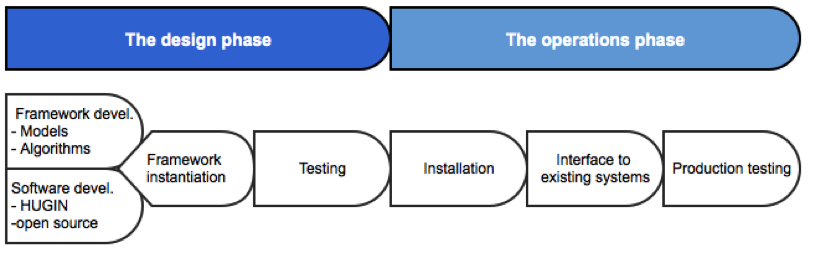
\includegraphics [keepaspectratio,width = 9cm] {figRe/REprocess2.png}\end{center}
\end{figure}
}
\end{frame}

\begin{frame} \frametitle{The AMIDST RE process} 
\vspace{-1cm}

\only<1->{
\begin{figure}
\begin{center}
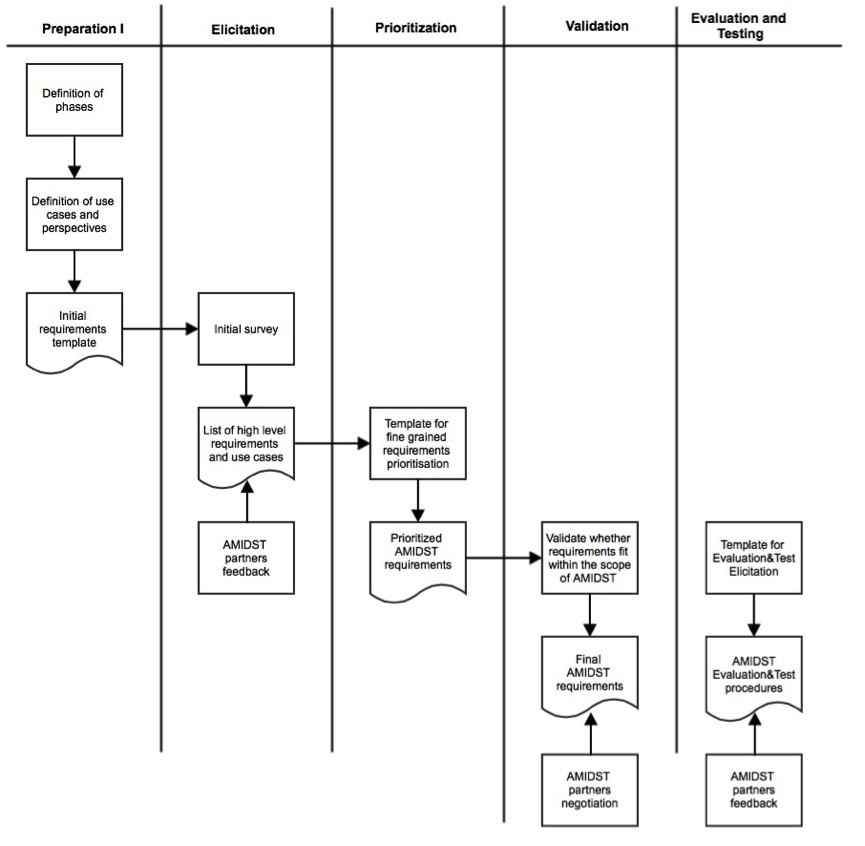
\includegraphics [keepaspectratio,width = 7cm] {figRe/REprocess1.png}\end{center}
\end{figure}
}
\end{frame}


%%%%%%%%%%%%%%%%%%%%%%%%%%%%%%%%%%%%
\section{Realization of the AMIDST RE process}
%%%%%%%%%%%%%%%%%%%%%%%%%%%%%%%%%%%%%

\begin{frame} \frametitle{Realization of the AMIDST RE process} 
\vspace{-1cm}
\begin{itemize}
\item<1-> Coupling between academic and industry partners
\item<2-> Formal template
\begin{itemize}
\item<2-> Simple description of RE
\item<2-> System description
\item<2-> Definition of user groups
\item<2-> Use cases
\item<2-> Requirements related to each use case
\end{itemize}
\item<3-> Requirements
\begin{itemize}
\item<3-> Linked to project phases
\item<3-> Linked to work packages
\item<3-> Prioritized in terms of must/should/could
\item<3-> Ranked in terms of importance
\end{itemize}
\end{itemize}
\end{frame}

\begin{frame} \frametitle{Realization of the AMIDST RE process} 
\vspace{-1cm}
\scriptsize{
\begin{table}[htbp]
  \centering
  \begin{tabular}{|c|c|c|c|c|}
    \hline
    Req.\ ID.\ & Relevant subphase & Must/should/could & Points & Task \\ \hline\hline
    DAI.U5.D1 & Framework devel.\ \& instan.\ & Should & 30 & 2.2  \\
    DAI.U5.D2 & Framework devel.\ \& instan.\ & Should & 20 & 2.2  \\
    DAI.U5.D3 & Framework devel.\ & Should & 15 & 2.2  \\
    DAI.U5.D4 & Framework devel.\ & Should & 15 & 2.2  \\
    DAI.U5.D5 & Framework instant.\ & Should & 20 & 2.2  \\
    DAI.U7.D1 & Framework devel.\ & Must & 35 & 2.1 \\
   \vdots & \vdots  & \vdots & \vdots & \vdots \\ \hline\hline
  \end{tabular}
  \caption{Example of work package requirements table}
\end{table}
}
\end{frame}


%%%%%%%%%%%%%%%%%%%%%%%%%%%%%%%%%%%%
\section{Conclusion}
%%%%%%%%%%%%%%%%%%%%%%%%%%%%%%%%%%%%

\begin{frame} \frametitle{Conclusion} 
\vspace{-1cm}
\begin{itemize}
\item<1-> RE process taylored to needs in AMIDST
\begin{itemize}
\item<1-> Pre-specified scope of the project
\item<1-> Very different stakeholders
\item<1-> Software need to be general enough for different industries
\end{itemize}
\item<2-> Realization of RE 
\begin{itemize}
\item<2-> Use case driven approach
\item<2-> Formal template across domains
\item<2-> Pairing of academic and industrial partners
\end{itemize}
\item<3-> Transfer to other projects 
\begin{enumerate}
\item<4-> Share the same characteristics
\item<5-> Reuse the very idea of identifying challenges to stear the RE process
\end{enumerate}
\end{itemize}
\end{frame}

%---------------------------------------------------------------------------------------------
\begin{frame} \frametitle{} 
{\it This project has received funding from the European Union's Seventh Framework Program for research, technological development and demonstration under grant agreement no 619209}
\end{frame}
%---------------------------------------------------------------------------------------------

\end{document}